\chapter{Cosmological perturbation theory}
\label{chap:perturbations}
In the previous chapters we mentioned several times that anisotropies and inhomogeneities are observed in our universe giving us a lot of information about it (section \ref{sec:LambdaCDM}). These deviations from the ideal homogeneous and isotropic FRW universe constitute tiny discrepancies (recall that for the CMB $\Delta T/T\approx 10^{-5}$) that can be studied as perturbations of the model we have built so far.
Clearly, a cosmological perturbation theory should account both for perturbations of the universe content and of its metric at the same time. Indeed, in general relativity any energy perturbation would affect the metric, perturbing it, which then would influence the evolution of the former.\\
Starting from a background metric $\bar g_{\mu\nu}(t)$, which only depends on time, we can introduce its perturbations $\delta g_{\mu\nu}(t, \mathbf x)$ as functions that we assume to be much smaller than the background and that also have some space dependence. Their dynamics is determined by plugging the perturbed metric in the Einstein field equations 
$$\bar G_{\mu\nu}+\delta G_{\mu\nu}=8\pi G\Big(\bar T_{\mu\nu}+\delta T_{\mu\nu}\Big),$$ where also the energy-momentum tensor has been perturbed for the reason we already explained. At this point the background part of the Einstein equations and the perturbed terms can be separated, since they do not mix at linear order, allowing to study first the background, which turns out to be just the Friedmann equations and thus gives FRW metric, and then its perturbations as a set of linear equations.
\section{Metric and matter perturbations}
\label{sec:perturbations}
To get simpler calculations, using conformal time, we can employ the following decomposition
\begin{align}
    g_{00}&=-a^2(\tau)\bigg[1+2A(\tau,\mathbf x)\bigg]\quad&\Rightarrow\qquad&\delta g_{00}=-2a^2(\tau)A(\tau,\mathbf x),\\
    g_{0i}&=a^2(\tau)B_i(\tau,\mathbf x)\quad&\Rightarrow\qquad&\delta g_{0i}=a^2(\tau)B_i(\tau,\mathbf x),\\
    g_{ij}&=a^2(\tau)\bigg[\delta_{ij}+h_{ij}(\tau,\mathbf x)\bigg]\quad&\Rightarrow\qquad&\delta g_{ij}=a^2(\tau)h_{ij}(\tau,\mathbf x).
\end{align} 
Each non-scalar perturbation in the above can be then further decomposed by studying its momentum space representation: consider first the vector $B_i$, in momentum space a natural direction is determined by the wave number vector $\mathbf k$ so that $B_i$ itself can be decomposed on such direction and on its orthogonal plane: $$B_i(\tau,\mathbf x)=\int\frac{d^3k}{(2\pi)^3}e^{i\mathbf{k\cdot x}}(ik_i\tilde B(\tau,\mathbf k)+\tilde{\hat{B}}_i(\tau,\mathbf x))=B_{,i}(\tau,\mathbf k)+\hat{B}_i(\tau,\mathbf x),$$ where we denoted with the hat the orthogonal components to $\mathbf{k}$. The above decomposition consists just in the split of the longitudinal, or irrotational, part $B_{,i}$ and the transverse, or solenoidal, part $\hat{ B}_i$ of a generic vector field. Indeed, it's rather trivial to note that $$\epsilon^{ijk}B_{,ij}(\tau,\mathbf x)=0\quad\text{and } \tensor{\hat B}{_{i}^{,i}}(\tau,\mathbf x)\propto\int\frac{d^3k}{(2\pi)^3}e^{i\mathbf{k\cdot x}}k^i\hat{B}_i(\tau,\mathbf x)=0.$$
The same decomposition can be used for $h_{ij}$: first we can factor out the trace, the remaining tensor is then projected in Fourier space on the direction of $\mathbf{k}$ and on its orthogonal plane in all the possible combinations of its indices. In this way we find:
$$h_{ij}(\tau,\mathbf x)=-2C\delta_{ij}+2E_{,ij}+\hat E_{i,j}+\hat E_{j,i}+\hat E^{T}_{ij},$$ where $C$ and $E$ are scalar fields, $\hat E_i$ is a transverse or solenoidal vector field while $\hat E^{T}_{ij}$ is a traceless transverse tensor.\\ Overall we found 10 fields which perfectly match the 10 degerees of freedom of the metric:
\begin{itemize}
    \item $A,B,C,E$ which are \textbf{scalar perturbations} with 1 degree of freedom each,
    \item $\hat B_i,\hat E_i$ which are \textbf{transverse vector perturbations}, thus with 2 degrees of freedom for each vector,
    \item $\hat E^T_{ij}$ which is a \textbf{traceless transverse tensor perturbation}, hence with just 2 degrees of freedom, and we recognize it to be a gravitational wave.
\end{itemize}

With the perturbed metric in our hands we can now study how the energy-momentum tensor of a perfect fluid gets perturbed. In the following discussion we will also generalize the universe content to an \emph{imperfect fluid} such as a combination different weakly interacting fluids, hence its energy-momentum tensor will include terms that describe physically relevant processes between its different components, for example the shear and bulk viscosity or the thermal conductivity. We can incorporate all of these effects in the \emph{shear stress} or \emph{anisotropic stress} $\pi^{\mu\nu}$, so that the general form of the energy-momentum tensor reads
\begin{equation}
    \tensor{T}{^\mu_\nu}=(\rho+p)U^\mu U_\nu+p\tensor{g}{^\mu_\nu}+\tensor{\pi}{^\mu_\nu}.
    \label{eq:Generalized_stress-energy_Tensor}
\end{equation}
Without loss of generality we can assume that $\pi^{\mu\nu}$ is traceless and flow-orthogonal, namely $\pi^{\mu\nu}U_\nu=0$ and $g_{\mu\nu}\pi^{\mu\nu}=0$. Indeed, from the above equation we can see that any non-traceless or flow-parallel contribution can be refactored in the energy density and in the pressure of the perfect fluid. This corresponds physically to require that in the rest frame of the fluid any shear stress is purely spatial, hence it manifests as an anisotropic contribution to the pressure ($\tensor{T}{^0_0}=\rho,\ \tensor{T}{^0_i}=0$ and $\tensor{T}{^i_j}=p\tensor{g}{^i_j}+\tensor{\pi}{^i_j}$). We now have to introduce perturbations in the above energy-momentum tensor: considering that $\pi^{\mu\nu}$ is already a deviation from the isotropic and homogeneous FRW case, we can assume that it is small enough to be treated as a perturbation, hence we still have to perturb the 4-velocity of the fluid $U^\mu$, the energy density and the pressure. \\ Starting from the 4-velcocity we assume that all its components could be perturbed, so that a small bulk velocity can appear ($U^i\neq0$): overall we will let $U^\mu=(\bar U^0+\delta U^0,\delta U^i)$, where $\bar U^0\gg\delta U^0,\delta U^i$ has the background value $a^{-1}$ that we get in the FRW case. Note that we can now define the bulk velocity of the fluid to be 
$$
v^i\defeq\frac{d x^i}{d\tau}=\frac{dx^i/d\lambda}{dx^0/d\lambda}=\frac{U^i}{U^0}=\frac{\delta U^i}{\bar U^0+\delta U^0}\approx \frac{\delta U^i}{\bar U^0}=a\delta U^i.
$$
The perturbation of the zeroth components can be found from the normalization condition which gives at first order
\begin{align*}
    -1=U^\mu U^{\nu}g_{\mu\nu}&=U^0U^0g_{00}+2U^0U^i g_{0i}+U^i U^j g_{ij}\approx -1+(\bar U^0)^2\delta g_{00}-2a^2\bar U^0\delta U^0\\
    \Rightarrow\quad U^0&=\frac{1}{a^3}\bigg(1-\frac{1}{2}\delta g_{00}\bigg),\qquad U_0=a^{-3}\bigg(1+\frac{1}{2}\delta g_{00}\bigg),
\end{align*}
while the spatial components are
$$U^i=\frac{1}{a}v^i\quad \Rightarrow\quad U_i=g_{ij}U^j+g_{0i}U^0\approx a\bigg(v_i+\frac{1}{a^2}\delta g_{0i}\bigg).$$
Let's stop for a moment to understand the physical meaning of this result: the zeroth component gets a perturbation that corresponds to the gravitational redshift of the energy of the fluid, while the spatial perturbation is the sum of a bulk velocity $\mathbf v$, that can arise due to the lack of isotropy, and a perturbation that we can interpret as the dragging of inertial frames at different velocities.\\
Similarly, also the energy density and the pressure get perturbed: considering their background values (those in FRW metric) $\bar\rho(t)$ and $\bar p(t)$ and some small deviations $\delta\rho(t,\mathbf x)$ and $\delta p(t,\mathbf x)$, we can write $\rho=\bar\rho+\delta\rho$ and $p=\bar p+\delta p$.\\ Plugging all the above perturbations in the energy-momentum tensor \eqref{eq:Generalized_stress-energy_Tensor} and keeping only the first order terms (assuming that all the perturbations are comparable) we find
\begin{align}
    \tensor{T}{^0_0}&=(\rho+p)U^0U_0+p\approx-(\bar\rho+\delta\rho)&\Rightarrow\quad &\delta \tensor{T}{^0_0}=-\delta\rho,\label{eq:perturbed_T00}&&\\
     \tensor{T}{^i_0}&=(\rho+p)U^iU_0\approx -(\bar\rho+\bar p)v^i&\Rightarrow\quad &\delta \tensor{T}{^i_0}=(\bar\rho+\bar p)v^i,\label{eq:perturbed_Ti0}&&\\
    \tensor{T}{^0_i}&=(\rho+p)U^0U_i\approx (\bar\rho+\bar p)\bigg(v_i+\frac{1}{a^2}\delta g_{0i}\bigg)&\Rightarrow\quad &\delta \tensor{T}{^0_i}=(\bar\rho+\bar p)\bigg(v_i+\frac{1}{a^2}\delta g_{0i}\bigg),\label{eq:perturbed_T0i}&&\\
    \tensor{T}{^i_j}&=(\rho+p)U^iU_j+p\tensor{g}{^i_j}+\tensor{\pi}{^i_j}\approx \bar p\tensor{\delta}{^i_j}+\tensor{\pi}{^i_j}  &\Rightarrow\quad &\delta \tensor{T}{^i_j}=\delta p\tensor{\delta}{^i_j}+\tensor{\pi}{^i_j}.\label{eq:perturbed_Tij}&&
\end{align} 
In this way we can come back to the perturbed Einstein equations and solve it separately for the background and for the perturbations.
\section{Gauge transformations}
The principle of general relativity states that the laws of physics are independent of the observer that describes them, hence they are independent of the coordinate that we use. In this section we will study how perturbations are influenced by a coordinate transformation. We will discover that the freedom of choice of the coordinates translates in a gauge freedom of the perturbations, reducing the number of degrees of freedom that are relevant.

Consider an infinitesimal coordinate transformation $x^\mu= \tilde x^\mu=x^\mu+\xi^\mu$, where $\xi^\mu$ is small vector field, comparable with the perturbations. This transformation will affect all the components of each tensor, in particular the metric will transform as
$$\tilde g_{\mu\nu}(\tilde x)=\frac{\partial x^\alpha}{\partial\tilde  x^\mu}\frac{\partial  x^\beta}{\partial\tilde x^\nu}g_{\alpha\beta}(x)=g_{\mu\nu}(x)-\frac{\partial \xi^\alpha}{\partial\tilde x^\mu}g_{\alpha\nu}(x)-\frac{\partial \xi^\beta}{\partial\tilde x^\nu}g_{\mu\beta}(x)+\mathcal O(\xi^2),$$
at this point it is useful to expand each term on the left-hand side around $\tilde x$, so that we get an expression depending only on the new coordinates $\tilde x^\mu$, which at first order reads:
$$\tilde g_{\mu\nu}(\tilde x)=g_{\mu\nu}(\tilde x)-\frac{\partial \xi^\alpha}{\partial \tilde x^\mu}g_{\alpha\nu}(\tilde x)-\frac{\partial \xi^\beta}{\partial \tilde x^\nu}g_{\mu\beta}(\tilde x)-\frac{\partial g_{\mu\nu}}{\partial \tilde x^\lambda}\xi^\lambda+\mathcal O(\xi^2).$$
Now we can separate the background and the perturbations and considering $\xi^\mu$ a first order perturbation we discover that the background metric remains unchanged, while each perturbation transforms as
\begin{equation}
     \delta \tilde g_{\mu\nu}(\tilde x)=\delta g_{\mu\nu}(\tilde x)-\frac{\partial \xi^\alpha}{\partial \tilde x^\mu}\bar g_{\alpha\nu}(\tilde x)-\frac{\partial \xi^\beta}{\partial \tilde x^\nu}\bar g_{\mu\beta}(\tilde x)-\frac{\partial\bar g_{\mu\nu}}{\partial \tilde x^\lambda}\xi^\lambda+\mathcal O(\xi^2,\delta g^2).
    \label{eq:perturbation_transformation}
\end{equation} 

The above transformation shows how the ten perturbation fields transforms under a change of coordinate. To better match the symmetries of the tensors we derived in the previous section, it is appropriate to decompose $\xi^\mu=(\xi^0,\zeta^{,i}+\xi^i_{\perp})$ where $\xi^0$ and $\zeta$ are two scalars while $\xi_\perp^i$ is a transverse vector ($\xi^i_{\perp,i}=0$).\\ The $00$ component gives us the transformation of the scalar perturbation $A$:
\begin{align}
    \delta \tilde g_{00}=-2a^2\tilde A=\delta g_{00}=- 2a^2 A+2a^2(\xi^{0})'+2aa'\xi^0\quad \Rightarrow\quad\boxed{\tilde A=A-\frac{1}{a}\frac{d}{d\tau}\bigg(a\xi^0\bigg)},\label{eq:gauge_A}
\end{align}
where we used the $'$ to denote the derivative with respect to conformal time.\\
Similarly, the $0i$ components give us the transformation of the vector perturbation $B_i$:
\begin{align*}
    \delta \tilde g_{0i}=a^2\tilde B_i=\delta g_{0i}=a^2B_i-a^2\tensor{\xi}{^j_{,0}}\delta_{ij}+a^2\tensor{\xi}{^0_{,i}} \Rightarrow\quad \tilde B_i=B_i-\xi_{i}'+\tensor{\xi}{^0_{,i}}.
\end{align*}
Decomposing both $\xi^i$ and $B_i$ in their longitudinal and transverse components we find
\begin{align}\label{eq:gauge_B}
    \tilde B=B-\zeta'+\xi^0,\qquad
    \tilde{\hat B}_i=\hat B_i-(\xi_{\perp i})'.
\end{align}
The same procedure goes for the $ij$ components
\begin{align*}\
    \delta \tilde g_{ij}=a^2\tilde h_{ij}=\delta g_{ij}=a^2h_{ij}-a^2\xi_{i,j}-a^2\xi_{j,i}-2aa'\xi^0\delta_{ij},
\end{align*}
again decomposing $h_{ij}$ in its scalar, vector and tensor components and comparing with the components of $\xi^\mu$ we find obtain the transformations of the remaining fields:
\begin{align}
    \tilde C&=C-\frac{a'}{a}\xi^0,&\quad
    \tilde E&=E-\zeta,\label{eq:gauge_CE}\\
    \tilde{\hat E}_i&=\hat E_i-\xi_{\perp i },&\quad
    \tilde{\hat E}^T_{ij}&=\hat E^T_{ij}.\label{eq:gauge_h}
\end{align} 
Let's stop for a moment to appreciate that the tensor perturbation is the only invariant perturbation under a change of coordinates. Other gauge invariant perturbations can be constructed from the above ones. For example writing the gauge parameters $\zeta$ and $\xi^0$ in terms of the perturbations,
$$ \zeta=  E-\tilde E,\qquad \xi^0=\tilde B-B +( E-\tilde E)',$$
a gauge invariant scalar perturbation can be obtained; by plugging $\xi^0$ in the transformation of $A$ and by rearranging the terms we find:
$$\tilde A+\frac{1}{a}(a\tilde E'-a\tilde B)'= A+\frac{1}{a}(a E'-a B)',$$ 
which shows that $\Phi_A\defeq A+\frac{1}{a}(a E'-a B)'$ is gauge invariant. Similarly, one can show that $\Phi_H\defeq -C+\frac{a'}{a}(B-E')$ is gauge invariant too. These two gauge invariant variables are called \emph{Bardeen variables}: note that these two variables represent the "real" (they are not coordinate artifacts) spacetime perturbations, since they cannot be removed by any change of coordinate.

Previously we argued that matter perturbations $\delta T_{\mu\nu}$ are related to the metric perturbations, therefore also this kind of perturbations possess the same gauge freedom.
To begin let's focus on the energy density and the pressure: under the transformation $\tilde x^\mu= x^\mu+\xi^\mu$ since they are scalars they won't transform, however the infinitesimal coordinate shift implies
$$\tilde\rho(\tilde x)=\rho(x)= \rho(\tilde x)-\xi^\mu\partial_\mu\rho(\tilde x)+\mathcal{O}(\xi^2).$$
By separating the background and the perturbed energy density and assuming that $\xi^\mu$ is comparable with $\delta\rho$, we discover again that the background energy density remains unchanged, while the perturbed one transforms as
$$ \delta\tilde\rho=\delta\rho-\xi^0\bar\rho'.$$
Analogously, pressure perturbations transform in the same way.\\
This immediately gives us the transformation for the $00$ component of the energy-momentum tensor \eqref{eq:perturbed_T00}:   
$$\delta \tilde T_{00}=-\delta\rho+\xi^0\bar\rho'=\delta T_{00}+\xi^0\bar\rho'.$$
To obtain the transformation of the other components we can use directly the transformation law of the energy-momentum tensor and then expand the old coordinates in terms of the new:
\begin{align*}
    \tensor{\tilde T}{^\mu_\nu}(\tilde x)&=\frac{\partial \tilde x^\mu}{\partial  x^\alpha}\frac{\partial x^\beta}{\partial  \tilde x^\nu}\tensor{T}{^\alpha_\beta}(x)=\tensor{T}{^\mu_\nu}(x)+\tensor{\xi}{^\mu_{,\alpha}}\tensor{T}{^\alpha_\nu}(x)-\tensor{\xi}{^\beta_{,\nu}}\tensor{T}{^\mu_\beta}(x)+\mathcal{O}(\xi^2)\\
    &=\tensor{T}{^\mu_\nu}(\tilde x)+\tensor{\xi}{^\mu_{,\alpha}}\tensor{T}{^\alpha_\nu}(\tilde x)-\tensor{\xi}{^\beta_{,\nu}}\tensor{T}{^\mu_\beta}(\tilde x)+\tensor{T}{^{\mu}_{\nu,\lambda}}(\tilde x)\xi^\lambda +\mathcal{O}(\xi^2).
\end{align*} 
Again by separating the background and the perturbed parts of energy-momentum tensor we find that the background part remains unchanged, while the perturbed part gets transformed as
$$\delta \tensor{\tilde T}{^\mu_\nu}=\delta \tensor{T}{^\mu_\nu}+\tensor{\xi}{^\mu_{,\alpha}} \tensor{\bar T}{^\alpha_\nu}-\tensor{\xi}{^\beta_{,\nu}} \tensor{\bar T}{^\mu_\beta}+\tensor{\bar T}{^{\mu}_{\nu,\lambda}}\xi^\lambda.$$
Note that from here we could have obtained the transformation of the $00$ component as well. The $i0$ perturbations transform as
\begin{align*}
    \delta  \tensor{\tilde T}{^i_0}&=-(\bar\rho+\bar p)\tilde v^i\\&=\delta \tensor{T}{^i_0}+\tensor{\xi}{^i_{,\alpha}}\tensor{\bar T}{^\alpha_0}-\tensor{\xi}{^\beta_{,0}}\tensor{\bar T}{^{i}_\beta}+\tensor{\bar T}{^{i}_{0,\lambda}}\xi^\lambda+\text{ $2^{nd}$ order terms}\\
    &=-(\bar \rho+\bar p)v^i-\bar\rho(\xi^i)'-\bar p \tensor{\delta}{^{i}_j}(\tensor{\xi}{^{j}})'+\text{ $2^{nd}$ order terms}\\&=-(\bar \rho+\bar p)[v^i+(\xi^i)'],
\end{align*}
which ultimately shows that $\tilde v^i=v^i+(\xi^i)'$ is the transformation of the bulk velocity.\\
The $ij$ components instead transform as
\begin{align*}
    \delta \tensor{\tilde T}{^i_j}&=\delta \tilde p\tensor{\delta}{^i_j}+\tensor{\tilde\pi}{^i_j}\\&=\delta \tensor{T}{^i_j}+\tensor{\xi}{^i_{,\alpha}}\tensor{\bar T}{^\alpha_j}-\tensor{\xi}{^\beta_{,j}}\tensor{\bar T}{^{i}_\beta}+\tensor{\bar T}{^{i}_{j,\lambda}}\xi^\lambda\\
    &=\delta p\tensor{\delta}{^i_j}+\tensor{\pi}{^i_j}+\bar p\xi^{i,j}-\bar p \tensor{\xi}{^{i,j}}+\bar \rho'\xi^0\\     
    &=\delta p\tensor{\delta}{^i_j}+\tensor{\pi}{^i_j}+\bar \rho'\xi^0,
\end{align*}
where we recognize the transformation of the pressure perturbation, hence showing that the shear stress $\pi^{ij}$ is gauge invariant.\\
Now that we know how the matter perturbations transform under an infinitesimal change of coordinate, we can try again to build a new gauge invariant variable. Assuming that the bulk velocity is an irrotational field, and thus it can be expressed as the gradient of a scalar field $v$, we can write its transformation as $\tilde v=v+\zeta'$, hence we can express $\zeta'$ as a function of $v$. Exploiting that $\tilde B=B-\zeta'+\xi^0$ we can write $\xi^0$ as a function of $B$ and $v$ which can be then substituted in the transformation of $C$ to get:
$$\tilde C+\frac{a'}{a}(\tilde B+\tilde v)=C+\frac{a'}{a}(B+v),$$
which shows that the variable $\mathcal{R}\defeq C+\frac{a'}{a}(B+v)$, called \emph{comoving curvature perturbation} is gauge invariant.

\subsection{Gauge choice}\label{sec:gauge_choice}
Having studied the gauge transformations of cosmological perturbations, it is now time to understand how to properly exploit this freedom to simplify our calculations. Our previous discussion already shows that in order to study tensor perturbations there is no gauge choice to make, since they are already gauge invariant. Vector perturbations, instead, are not excited during inflation, hence we will focus on scalar perturbations.
\begin{itemize}
    \item The first gauge choice we present is the \textbf{Newtonian gauge}: this is defined by the condition that the fields $B$ and $E$ vanish identically. This is accomplished by an infinitesimal change of coordinates with $\zeta = E$ and $\xi^0=E'-B$, which sets $\tilde E=\tilde B=0$. The perturbed metric in this way reads 
    \begin{equation}
    ds^2=a^2(\tau)\bigg[-(1+2\Psi)d\tau^2+(1-2\Phi)\delta_{ij}dx^idx^j\bigg],
    \end{equation}
    where we redefined $\Psi\defeq A$ and $\Phi\defeq -C$ and no other scalar perturbation is required to fully describe the system. This gauge choice is particularly important since it makes the metric diagonal, allowing to have geodesic motion orthogonal to constant time hypersufaces and simplifying many calculations. Furthermore, the form of the metric allows recognizing $\Psi$ as the gravitational potential that appears in the weak field limit of general relativity. Lastly, it is very important to note that by imposing $B=E=0$, the two Bardeen variables reduces to $\Psi$ and $\Phi$, showing that this gauge choice automatically removes all the coordinate artifacts that could be confused with perturbations.
    \item    Another convenient gauge choice is the \textbf{spatially flat gauge}, defined by $C=E=0$. This condition removes any scalar perturbation from the spatial part of the metric, however in this case we are left with a non-diagonal metric which is not convenient in many calculations.
    \item
    Historically introduced by Lifshitz as one of the first gauge choices, the \textbf{synchronous gauge} is defined by the condition $A=B=0$. However, this gauge presents many complications that led to the development of the Newtonian gauge.
    \item
    As we already discussed, also matter perturbations are affected by infinitesimal coordinate transformations, this implies that some gauge choice are available also by imposing conditions on the energy-momentum tensor. The main gauge choice of this kind is the \textbf{comoving gauge}, defined by the condition $\delta \tensor{T}{^0_i}=0$, physically corresponds to the choice of the comoving reference frame with respect to the perturbed cosmic fluid. The above condition corresponds to 
    $$0=\delta \tensor{T}{^0_i}=(\bar\rho+\bar p)(v_i+B_i),$$
    that assuming an irrotational bulk velocity translates into $B+v=0$. In this gauge we are allowed to impose an extra condition since $B+v=0$ is achieved just by using $\xi^0$, hence we are still free to use $\zeta$ to set $E=0$. In this way the only purely spatial scalar perturbation that remains is $\mathcal{R}$. Moreover, studying the equation of motion for $A$ and $B$, one can show that these become auxiliary fields which can be expressed as combinations of other perturbations or background fields. In this way the only relevant scalar perturbation to be studied in this gauge is just the comoving curvature $\mathcal{R}$.
\end{itemize} 
\section{Initial conditions}
\label{sec:initial_condition}
In the previous sections we described how to build the perturbation theory that can capture the evolution of anisotropies which we observe in our universe. Even though we still haven't derived the equation of motion for these, we already explained that they are given by the perturbed Einstein field equations. In the end these result in a system of linear differential equations that, in order to be solved, needs a set of initial conditions. We will see that initial conditions are given by inflation (which however was theorized in order to solve other problems in the \emph{hot big bang model}) by exploiting the quantum fluctuations of the vacuum on a curved background.

Even though we still don't know the origin of such conditions, we can classify them. The most important one is the \textbf{adiabatic initial condition}, which corresponds to the requirement that initially all the components of the cosmic fluid do not exchange heat among themselves. How this requirement gives an initial condition can be understood just by considering the \emph{first law of thermodynamics} in a small volume of fluid:
\begin{align*}
    TdS_i=dU_i+p_idV=\rho_idV+Vd\rho_i+p_idV \quad\Rightarrow\quad T\frac{dS_i}{V}=d\rho_i+(\rho_i+p_i) \frac{dV}{V},
\end{align*}
where the subscript $i$ indicates that we are considering the thermodynamical variable of one component of the cosmic fluid. Given the assumption that $dS_i=0$ for all components and since the volume and its variation is the same for all, the above relation tells us that the ratio $\frac{\rho_i}{\rho_i+p_i}$ is the same for all the spices. Furthermore, assuming that the usual equation of state ($p=\omega\rho$) holds and approximating the $\delta\rho\approx d\rho$, we find
$$\frac{\delta \rho_i}{\rho_i}\frac{1}{1+\omega_i}=\frac{\delta \rho_j}{\rho_j}\frac{1}{1+\omega_j}\qquad\text{for all } i,j.$$
In the $\Lambda$CDM model we have mainly four components: photons and neutrinos, with $\omega=1/3$, cold dark matter and regular matter, with $\omega=0$. In this case the adiabatic condition translates into
\begin{equation}
    \frac{\delta \rho_\gamma}{\rho_\gamma}=\frac{\delta \rho_\nu}{\rho_\nu}=\frac{4}{3}\frac{\delta \rho_\text{CDM}}{\rho_\text{CDM}}=\frac{4}{3}\frac{\delta \rho_\text{b}}{\rho_\text{b}},
\end{equation}
which allows obtaining all the initial conditions from just one matter perturbation.

Other conditions, such as the \textbf{isocurvature initial conditions}, exits but both theoretically and observationally they seem to be less relevant than the adiabatic one. Indeed, the most simple models of inflation shows a good agreement with this kind of conditions, mainly because its dynamics in a single patch of universe it is fully determined by just one inflaton field. Moreover, current observation of the CMB further confirm the validity of the adiabatic initial condition.  

\section{Primordial perturbations}
As we mentioned, the initial conditions of the perturbations are determined by inflation. In the followinf sections we will discover that perturbations naturally arise from quantum mechanics in curved spacetime as the inflaton field dominates the universe. The accelerated inflationary expansion stretched these perturbations from the quantum scale to the Hubble scale where, as we will see, they freeze and become classical. Then transitioning to the radiation dominated era the pertirbations start to renter the Hublle horizon, where they start to evolve again. In this way the initial conditions are determined by the perturbations at the Hubble scale during inflation. 
\subsection{Scalar perturbations during inflation}
In Chapter \ref{chap:inflation} we developed the general framework that describes inflation: this was done by assuming that the inflaton can be described as a quantum fields which is totally homogeneous and depends only on the time variable. In this section we will allow for perturbation to introduce a space dependece in the inflaton field. As usual we will split the filed in its backgorund component $\bar\phi(\tau)$ plus some small perturbation $\delta\phi(\tau,\mathbf x)$.

The starting point is the action of a scalar field, minimally coupled to gravity
$$\mathcal{S} [g,\phi]=-\int d^4x\sqrt{-g}\bigg(\frac{1}{2}\partial_\mu\phi\partial^\mu\phi+V(\phi)-\frac{R}{16\pi G}\bigg),$$where $R$ is the Ricci scalar. Since we want to study inhomogeneities, we perturb both the metric, in the way we explained in Section \ref{sec:perturbations}, and the inflaton field, which now is our universe content. Let us stop for a moment and consider the perturbed energy-momentum tensor of the inflaton: expanding at the first order in all perturbations we find
\begin{align*}
    \tensor{T}{^0_i}=\partial^\mu\phi\partial_\nu\phi+\tensor{g}{^0_i}\mathcal{L}=-a^{-2}\bar\phi'\delta\phi_{,i},
\end{align*}
where we used the perturbed metric with conformal time in the Newtonian gauge. This shows that the comoving gauge ($\delta\tensor{T}{^0_i}=0$) corresponds to the reference frame in which the inflaton is unperturbed $\delta\phi=0$.
Using the ADM formalism one can show that, in this gauge, scalar perturbations are parametrized only by the comoving curvature $\mathcal{R}$, despite the metric still containing $A$ and $B$:
$$ds^2=-a^2(1+2A)d\tau^2+2a^2B_{,i}d\tau dx^i+a^2(1-2\mathcal{R})\delta_{ij}dx^idx^j.$$
Indeed, as we already explained in Section \ref{sec:gauge_choice} these two last fields reduce to auxiliary fields. For these reasons we fix the comoving gauge from now on.\\
Through the ADM formalism one can also show that the above action, at the second order reads
\begin{equation}
    \mathcal{S}_{2}[\mathcal{R} ]=\frac{1}{2}\int d^4x a^4\bigg(\frac{\bar \phi'}{a'}\bigg)^2\Big[(\mathcal{R}')^2-(\mathcal{R}_{,i})^2\Big].
\end{equation}
Even though $\mathcal{R}$ has many useful proprieties, it is immediately clear that it is not the canonical variable of this system and, since we aim to quantize these fields, we must find a proper canonical one. The appropriate choice is the so-called \textbf{Mukhanov-Sasaki variable}
\begin{equation}
    \sigma\defeq z\mathcal{R},\quad \text{with }z\defeq=a^2\frac{\bar\phi'}{a'}=a^2\frac{\dot{\bar\phi}}{\dot{a}}=a\frac{\dot{\bar\phi}}{H},\label{eq:SM-variable}
\end{equation}
that with some simple algebra turns the previous action into
\begin{equation}
    \mathcal{S}_{2}[\sigma ]-\frac{1}{2}\int d^4x \Big[(\sigma')^2+\frac{z''}{z}\sigma^2-(\sigma_i)^2\Big].   \label{eq:SM-action}
\end{equation}
Euler-Lagrange equations then give the \textbf{Mukhanov-Sasaki equation}
\begin{equation}
    \sigma''-\bigg(\boldsymbol{\nabla}^2\sigma+\frac{z''}{z}\bigg)\sigma=0,\label{eq:SM-equation}
\end{equation}
which we can recognize to be the Klein-Gordon equation with an effective time-dependent mass $m_\text{eff}=-z''/z$.

We are now interested in quantizing the Mukhanov-Sasaki variable: the similarity between the Minkowskian Klein-Gordon equation and equation \eqref{eq:SM-equation} allows for a similar procedure to be followed. First we compute the conjugate momentum, $\pi= \partial\mathcal{L} /\partial \sigma'=\sigma'$, which will be then promoted to be an operator by imposing canonical commutation relations
\begin{align*}
    [\hat\sigma(\tau,\mathbf x),\hat\sigma'(\tau,\mathbf y)]=i\delta^{(3)}(\mathbf{x-y}),\qquad  [\hat\sigma(\tau,\mathbf x),\hat\sigma(\tau,\mathbf y)]= [\hat\sigma'(\tau,\mathbf x),\hat\sigma'(\tau,\mathbf y)]=0.
\end{align*}
More in detail, this is accomplished by studying equation \eqref{eq:SM-equation} in Fourier space, where it reads
$$\tilde\sigma_\mathbf{k}''+\bigg(\mathbf k^2-\frac{z''}{z}\bigg)\tilde\sigma_\mathbf{k}=0,$$
then the Fourier coefficient of each mode is promoted to an operator. Note that $\sigma_\mathbf{k}$ depends only on the modulus of $\mathbf k$, hence we will drop the bold notation to signal this dependence. In this way the whole quantum field will read
$$\hat\sigma(\tau\,\mathbf{x})=\int\frac{d^3k}{(2\pi)^3}\bigg[\hat a_{\mathbf k}\tilde\sigma_k(\tau)e^{i\mathbf{k\cdot x}} +\hat a_{\mathbf k}^{\dagger}\tilde\sigma^*_k(\tau)e^{-i\mathbf{k\cdot x}}\bigg],$$
where the different signs in the exponentials are due to the requirement that $\hat\sigma^\dagger=\hat\sigma$, as $\sigma\in\mathbb{R}$ before the quantization, and both $\tilde\sigma_k$ and $\tilde\sigma_k*$ are included since they are linearly independent solutions. The operator $\hat a_\mathbf{k}$ and $\hat a^\dagger_\mathbf{k}$ are called \textbf{creation and annihilation operators} and they are defined through the commutation relations $$[\hat a_\mathbf{k},\hat a^\dagger_\mathbf{k'}]=(2\pi)\delta^{(3)}(\mathbf{k-k'}),\quad [\hat a_\mathbf{k},\hat a_\mathbf{k'}]=[\hat a^\dagger_\mathbf{k},\hat a^\dagger_\mathbf{k'}]=0.$$ These relations allow obtaining the canonical commutation relations precisely if the following normalization holds
\begin{align*}
&\qquad\qquad\qquad\langle\sigma_k,\sigma_k\rangle=i(\tilde\sigma^*_k\tilde\sigma'_k-(\tilde\sigma_k^*)'\tilde\sigma_k)=1\\ [\hat\sigma(\tau,\mathbf x),\hat\sigma'(\tau,\mathbf y)]&=\int\frac{d^3k}{(2\pi)^3}\frac{d^3k'}{(2\pi)^3}    \Big([\hat a_\mathbf{k},\hat a^\dagger_\mathbf{k'}]\tilde\sigma_k(\tilde\sigma^*)'_{k'}e^{i(\mathbf{k\cdot x-k'\cdot y})}+[\hat a^\dagger_\mathbf{k},\hat a_\mathbf{k'}]\tilde\sigma_k^*\tilde\sigma'_ke^{-i(\mathbf{k\cdot x-k'\cdot y})}\Big)\\&=-\int\frac{d^3k}{(2\pi)^3}e^{i\mathbf{k\cdot(x-y)}}    (\tilde\sigma^*_k\tilde\sigma'_k-(\tilde\sigma_k^*)'\tilde\sigma_k)=i\delta^{(3)}(\mathbf{x-y}).
\end{align*}
Lastly, quantum states are defined by the action of the creation and annihilation operators: first the vacuum state $\ket{0}$, then 1-particle states $\ket{1_\mathbf{k}}$ and so on:
\begin{equation}
    \ket{0}\text{ such that }\hat{a}_\mathbf{k}\ket{0}=0\ \forall \mathbf{k},\qquad \ket{1_\mathbf{k}}\defeq\hat{a}^\dagger_\mathbf{k}\ket{0}.
\end{equation}
Notice that this whole construction is not unique as the basis of solutions of the Mukhanov- Sasaki equation is not unique: indeed the lack of the symmetries, such as the Poincare Group, prevents us to recognize a preferred basis (in contrary to what happens in flat spacetime with normal modes). Different basis are connected by \emph{Bogoliubov transformations} (a detailed treatment of quantum field theory in curved spacetime can be found in \cite{Birrell:1982ix}), which also link the different quantum field theories that correspond to each basis. The choice of the appropriate basis is fundamental to describe the right quantum field theory: in our case we will study the limit in which the curvature  of spacetime is negligible and require that there the Minkowski construction is recovered. This choice will give us the so-called \textbf{Bunch-Davies} modes and its associated vacuum state $\ket{0_\text{BD}}$.

To conclude our quantum approach to inflation we want to study the observable that emerge from the quantum mechanical operators. Trivially, we can observe that the expectation value of the Mukhanov-Sasaki variable, for the vacuum state, is zero:
$$\braket{0_\text{BD}|\hat{\tilde\sigma}_\mathbf{k}|0_\text{BD}}=\braket{0_\text{BD}|\hat a_{\mathbf k}\tilde\sigma_k+\hat a_{-\mathbf k}^{\dagger}\tilde\sigma^*_{-k}|0_\text{BD}}=0.$$
On the other hand, its variance is non-zero and it is given by the so-called \textbf{power spectrum}:
\begin{align*}
   &\braket{0_\text{BD}|\hat{\tilde\sigma}_\mathbf{k}\hat{\tilde\sigma}_\mathbf{k'}|0_\text{BD}}=\\ &\qquad=\braket{0_\text{BD}|\hat a_{\mathbf k}\hat a_{\mathbf k'}\tilde\sigma_k \tilde\sigma_{k'}+\hat a_{\mathbf k}\hat a_{-\mathbf k'}^{\dagger}\tilde\sigma_{k} \tilde\sigma^*_{k'}+\hat a_{-\mathbf k}^{\dagger}\hat a_{\mathbf k'}\tilde\sigma_{-k}^* \tilde\sigma_{k'}+\hat a_{-\mathbf k}^\dagger\hat a_{-\mathbf k'}^{\dagger}\tilde\sigma_{-k} \tilde\sigma^*_{-k'}|0_\text{BD}}\\&\qquad=\braket{0_\text{BD}|\hat a_{\mathbf k}\hat a_{-\mathbf k'}^{\dagger}|0_\text{BD}}\tilde\sigma_{k} \tilde\sigma^*_{k'}=|\tilde\sigma_{k}|^2\delta^{(3)}(\mathbf{k+k'})\defeq\mathcal{P}_{\sigma}(k)\delta^{(3)}(\mathbf{k+k'}).
\end{align*} 
Physically this means that during inflation the scalar perturbations, even if not present in the first place, can be sourced by vacuum fluctuations. In this way we manage to build initial conditions for the perturbed Einstein equations that we previously discussed.

At this point the only thing that remains to be found are the Bunch-Davies modes. First, we should find solutions for the Mukhanov-Sasaki equation in momentum space, for which the background evolution of inflation must be known. In the following we will work with slow-roll inflation but in general more complex models can be used. As we already noted equation \eqref{eq:SM-equation} contains an effective mass $-z''/z$ which is time dependent, hence to find its solution this dependence must be addressed. Using equation \eqref{eq:SRP_field},
$$\epsilon_1=4\pi G\frac{\dot{\bar\phi}^2}{H^2}\qquad \Rightarrow\qquad z\defeq a\frac{\dot{\bar\phi}}{H}=a\sqrt{\frac{\epsilon_1}{4\pi G}},$$
 and differentiating twice $z$, with some simple algebra the effective mass can be express as a function of the slow-roll parameters: 
$$z'=aHz\Big(1+\frac{\epsilon_2}{2}\Big),\quad z''=z(aH)^2\bigg(2-\epsilon_1+\frac{3}{2}\epsilon_2- \epsilon_1\epsilon_2+\frac{(\epsilon_2)^2}{4}+\frac{\epsilon_2\epsilon_3}{2}\bigg),$$
where $\epsilon_i\defeq \dot{\epsilon}_{i-1}/(H\epsilon_{i-1})$ for $i\geq 2$.
Then, considering that inflation occurs in quasi-De Sitter spacetime, we can approximate the factor $(aH)^2$ in the following way
$$\frac{d}{d\tau}\frac{1}{aH}=\epsilon_1-1\quad \Rightarrow\quad aH\approx\frac{1}{\tau(\epsilon_1-1)}\approx-\frac{1}{\tau}(1+\epsilon_1),$$
Plugging these results in the Mukhanov-Sasaki equation and introducing $\nu$ we can write
\begin{equation}
    \tilde\sigma_k''+\bigg[\mathbf k^2-\frac{1}{\tau^2}\bigg(\nu^2-\frac{1}{4}\bigg)\bigg]\tilde\sigma_k=0,\quad\text{where}\quad\nu^2\defeq \frac{9}{4}+3\epsilon_1+\frac{3}{2}\epsilon_2,\label{eq:SM_Slowroll}
\end{equation}
where we only kept terms at the first order in the slow-roll parameters. The solutions to this equation are the \emph{Hankel functions} of the first kind $H_\nu^{(1)}$ and of the second kind $H_\nu^{(2)}$, so that in general
$$\tilde\sigma_k(\tau)=\sqrt{-\tau}\big(C_1H_\nu^{(1)}(-k\tau)+C_2H_\nu^{(2)}(-k\tau)\big),$$ which is defined up to the two constants $C_1$ and $C_2$. The Bunch-Davies condition gives us a way to determine these coefficients: modes whose wavelengths are much smaller than comoving Hubble horizon, $\mathbf k^2\gg1/\tau^2\approx(aH)^2$, experience flat Minkowski spacetime since the curvature of spacetime becomes negligible. Indeed, in this limit the modes are expected to behave as in flat Minkowski spacetime as the equation \eqref{eq:SM_Slowroll} reduces to Klein-Gordon. Physically this corresponds to an early-time limit, in which inflation has still not stretched the perturbations outside the Hubble horizon. Considering $k\tau\to-\infty$ the Hankel functions can be approximated as
\begin{align*}
    H_\nu^{(1)}(x)\xrightarrow{x\to\infty}\sqrt{\frac{2}{\pi x} }e^{i\big(x-\frac{\pi}{2}\nu-\frac{\pi}{4}\big)},\qquad H^{(2)}_\nu(x)\xrightarrow{x\to\infty}\sqrt{\frac{2}{\pi x} }e^{-i\big(x-\frac{\pi}{2}\nu-\frac{\pi}{4}\big)},
\end{align*}
which shows that the Bunch-Davies condition is satisfied if 
$$\lim_{k\tau\to -\infty}\tilde\sigma_k=\frac{e^{ik\tau}}{\sqrt{2k}}\qquad\Longleftrightarrow\qquad C_1=0\text{ and }C_2= \sqrt{\frac{\pi}{4}}.$$
We conclude that the right modes to use are 
\begin{equation}
    \tilde\sigma_k(\tau)=\sqrt{-\tau}\sqrt{\frac{\pi}{4}}H_\nu^{(2)}(-k\tau).\label{eq:sigma_BD_mode}
\end{equation}

The so-called \textbf{sub Hubble horizon regime} $k^2\gg(aH)^2$ has just been exploited to find the Bunch-Davies modes; its opposite limit $k^2\ll(aH)^2$ is called \textbf{super Hubble horizon regime}, and physically it corresponds to a late-time limit in which many modes have been already stretched outside the Hubble horizon. In this limit equation \eqref{eq:SM_Slowroll} reduces to a much simpler form, that by neglecting the slow-roll parameters reads
$$ \tilde\sigma_k''-\frac{2}{\tau^2}\tilde\sigma_k=0\quad\xrightarrow{\text{ansatz }\tilde\sigma_k\propto \tau^p}\quad\tilde\sigma_k=\frac{C_1}{\tau}+C_2\tau^2.$$
However $\sigma$ is not a metric perturbation and, to obtain a physical quantity, $\mathcal{R}$ should be considered. Recalling that $\sigma=\mathcal{R}z$ and using the expression for $z'$ we derived, we find that the comoving curvature perturbation at the super Hubble horizon scale become frozen and stops evolving:
\begin{align*}
    z'\approx zaH\approx-\frac{z}{\tau}\quad\Rightarrow\quad z(\tau)\approx\frac{1}{\tau}\quad\Rightarrow\quad\tilde{\mathcal{R}}_k\approx C_1+C_2\tau\xrightarrow{\tau\to 0}C_1,
\end{align*}
where the last limit is exactly the super Hubble horizon regime $aH\to\infty$. Hence, the only information that we will need to obtain the initial condition for cosmological perturbations is the power spectrum in the late-time limit, which, until the modes reenter the Hubble horizion, is time independent.

For these reasons we will not study the power spectrum of $\sigma$ but rather the one of the comoving curvature $\mathcal{R}$, which is:
$$\mathcal{P_R}(k)=\frac{\mathcal{P}_\sigma}{z^2} =\frac{|\sigma_k|^2}{z^2}=-\tau8\pi G\frac{\pi}{8a^2\epsilon_1}|H_\nu^{(2)}(-k\tau)|^2,$$where we used that $z=a\sqrt{\epsilon_1/(4\pi G)}$. In the super Hubble horizon limit the Hankel function can be approximated as 
$$|H_\nu^{(2)}|^2\xrightarrow{k\tau\to0}\frac{2^{2\nu}\Gamma^2(\nu)}{\pi^2}(-k\tau)^{-2\nu}\xrightarrow{\nu\approx3/2}\frac{2}{\pi}\bigg(\frac{k}{aH}\bigg)^{-2\nu},$$ where $\Gamma$ is the gamma function and $\Gamma^2(3/2)\approx\pi/2$ while $\tau\approx-(aH)^{-1}$. In this way the power spectrum reads
\begin{equation}
    \mathcal{P_R}(k)=8\pi G\frac{H^2}{4\epsilon_1(aH)^3}\bigg(\frac{k}{aH}\bigg)^{-2\nu},\label{eq:Scalar_Power_spectrum}
\end{equation}
This quantity is usually expressed as the \textbf{dimensionless power spectrum}
\begin{equation}
    \Delta_\mathcal{R}(k)\defeq \frac{k^3}{2\pi^2}\mathcal{P_R}(k)=8\pi G\frac{H^2}{8\pi^2\epsilon_1}\bigg(\frac{k}{aH}\bigg)^{3-2\nu}.\label{eq:Scalar_Dimensionless_Power_spectrum}
\end{equation}

\subsection{Tensor perturbations during inflation}
Following the same ideas that guided us in the previous section, we shall now study the dynamics of the tensor perturbations $\hat E_{ij}^T$ during inflation. Since we are going to consider only tensor modes, we will use $h_{ij}$ to denote transverse traceless perturbations of the spatial components of the metric. While studying these perturbations, scalar perturbations (since overall perturbation theory gives a system of linear PDE) are decoupled and thus an action only for $h_{ij}$ can be considered. Starting from the Hilbert-Einstein action the ADM formalism can be used to obtain
\begin{equation}
    \label{eq:tensor_perturb_action}
    \mathcal{S} [h_{ij}]=\frac{1}{64\pi G}\int d^4xa^2\Big[(h'_{ij})^2-(h_{ij,k})^2\Big]=\frac{1}{64\pi G}\sum_{\lambda=+,\times}\int d^4xa^2\Big[(h'_{(\lambda)})^2-(h_{(\lambda),k})^2\Big],
\end{equation}
where we used the decomposition of gravitational waves in their two polarizations (the detail of the propagation of gravitational waves will be explained in Section \ref{sec:free_GW})
$$h_{ij}=\sum_{\lambda=+,\times}h_{(\lambda)}\boldsymbol\epsilon^\lambda_{ij}\qquad \text{with }\boldsymbol{\epsilon}^\lambda_{ij}\boldsymbol{\epsilon}^{\lambda}_{ij}=1.$$
The above action shows that also in this case $h^{(\lambda)}$ is not the canonical variable of this system: it is easy to note that the right canonical variable is $\sigma_{(\lambda)}\defeq ah_{(\lambda)}/(2\sqrt{2\pi G})$ and with some little algebra the above action becomes
\begin{equation}
    \mathcal{S} [h_{ij}]=\frac{1}{2}\sum_{\lambda=+,\times}\int d^4x\Big[(\sigma'_{(\lambda)})^2+\frac{a''}{a}\sigma_{(\lambda)}^2-(\sigma_{(\lambda),k})^2\Big],
\end{equation}
which we recognize to be exactly the Mukhanov-Sasaki action \eqref{eq:SM-action} but with an effective mass that now is a function solely of the scale factor.

To solve the associated equation of motion, the effective mass must be computed explicitly as a function of conformal time: starting from the derivative of the Hubble horizon we find in the slow-roll approximation
$$\frac{d}{d\tau}\frac{1}{aH}=\epsilon_1-1\quad\Rightarrow\quad \frac{a'}{a}=aH\approx-\frac{1+\epsilon_1}{\tau}\quad\Rightarrow\quad\frac{a''}{a}\approx\frac{2+3\epsilon_1}{\tau^2},$$
hence the equation of motion for the above action reads for each mode
\begin{equation}
    \sigma''_{(\lambda)}-\boldsymbol\nabla^2\sigma_{(\lambda)}-\frac{1}{\tau^2}\bigg(\nu_T^2-\frac{1}{4}\bigg)\sigma_{(\lambda)}=0,\quad\text{where }\nu_T^2\defeq\frac{9}{4}+3\epsilon_1.
\end{equation}
This equation is exactly the Mukhanov-Sasaki equitation \eqref{eq:SM_Slowroll} with a different $\nu$ and therefore we won't need any further calculation that hasn't already been done in the previous section. The modes of each polarization are again the Hankel functions with the same normalization we obtained through the Bunch-Davies condition:
$$\tilde\sigma_{k(\lambda)}=\sqrt{-\tau}\sqrt{\frac{\pi}{4}}H_{\nu_T}^{(2)}(-k\tau).$$
Also for tensor modes we note that at super Hubble horizon scale these freeze: indeed $\tilde\sigma_{k,(\lambda)}$ is a combination of the two solutions $ \tau^{-1}$ and $\tau^2$. A simple calculation in quasi-De Sitter space gives $a\propto\tau$, which result in two solutions for $\tilde h_{k,(\lambda)}\propto a\tilde\sigma_{k,(\lambda)}$: a constant one (given by $\tau^{-1}\times\tau$) and a decaying one (given by $\tau^2\times\tau$).
 
At this point, if we were to quantize the field $\sigma_{(\lambda)}$ we would have obtained the same results of the scalar case for each polarization: a zero expectation value and a variance determined by the power spectrum. Knowing that the physical observable, which moreover does not evolve at superhorizion scales, is $h_{(\lambda)}$ we want to find its power spectrum
\begin{align*}
    \mathcal{P}_T(k)&\defeq\braket{0_\text{BD}|\hat{\tilde h}_{ij}\hat{\tilde h}_{ij}|0_\text{BD}}=\frac{16\pi G}{a^2}\sum_{\lambda=+,\times}\braket{0_\text{BD}|\hat{\tilde\sigma}_{\mathbf(\lambda)}\hat{\tilde\sigma}_{\mathbf(\lambda)}|0_\text{BD}} \\&=32\pi G\sum_{\lambda=+,\times}\frac{|\tilde\sigma_{k(\lambda)}|^2}{a^2}=64\pi^2 G\frac{|H_{\nu_T}^{(2)}|^2}{4a^3H},
\end{align*}
where an extra factor $\times 2 $ appears since both polarizations contribute equally. Recalling the super Hubble horizon limit of the Hankel function
\begin{equation}
    |H_{\nu_T}^{(2)}(-k\tau)|^2\xrightarrow{k\tau\to 0}\frac{2^{2\nu_T}\Gamma^2(\nu_T)}{\pi^2}(-k\tau)^{-2\nu_T}\xrightarrow{\nu_T\approx3/2}\frac{2}{\pi}\bigg(\frac{k}{aH}\bigg)^{-2\nu_T},
\end{equation}
we find the power spectrum and the dimensionless power spectrum, respectively:
\begin{equation}
    \mathcal{P}_T(k)=\frac{32\pi G}{a^3H}\bigg(\frac{k}{aH}\bigg)^{-2\nu_T},\qquad\Delta_h(k)\defeq\frac{k^3}{2\pi^2}\mathcal{P}_T(k)=8\pi G\frac{2H^2}{\pi^2}\bigg(\frac{k}{aH}\bigg)^{3-2\nu_T}.\label{eq:tensor_power_spectrum}
\end{equation}
\subsection{Phenomenology of the power spectrum}
In the previous two sections we obtained the power spectra of primordial scalar and tensor perturbations at the super Hubble horizon scale: in both cases we discovered that the power law is the form of slow-roll inflation power spectra. For each power spectra two quantities are defined: the \emph{amplitude} $\mathcal A$ and the \emph{spectral index} or \emph{tilt} $n$, which are the two quantities that we measure from observations. In general the two power spectra are then expressed as
\begin{equation}
    \Delta_\mathcal{R}(k)=\mathcal{A_R}\bigg(\frac{k}{k_0}\bigg)^{n_s-1}\qquad\text{and}\qquad\Delta_T(k)=\mathcal{A}_h\bigg(\frac{k}{k_0}\bigg)^{n_t},
\end{equation}
where $k_0$ is called \emph{pivot scale} and defines the scale at which the power spectrum exactly equals to its amplitude. Note that in this way, while the tilt is independent of the pivot scale, the amplitude depends on $k_0$ since any rescale of this could be reabsorbed in $\mathcal A$.\\ From equations \eqref{eq:Scalar_Dimensionless_Power_spectrum} and \eqref{eq:tensor_power_spectrum} we recognize at the Hubble horizon scale
\begin{equation}
    \mathcal{A_R}=8\pi G\frac{H^2}{8\pi^2\epsilon_1},\ n_s=1-2\epsilon_1,\quad\text{and}\quad\mathcal{A}_T=8\pi G\frac{2H^2}{\pi^2},\ n_t=-2\epsilon_1.
\end{equation}
The above quantities imply that a \emph{consistency} relation should hold between their respective power spectra: indeed, defining the \textbf{tensor-to-scalar ratio}
\begin{equation}
    r(k)\defeq\frac{\mathcal{P}_T(k)}{\mathcal{P_R}(k)},
\end{equation} 
in the slow-roll approximation of a single field inflation, $r=16\epsilon_1=-8n_t$. Deviations from this relation signal that inflation is not driven by a single quantum inflaton field. While the CMB anisotropies allowed to characterize with good precision the power spectrum of primordial scalar perturbations, $\mathcal{A_R}=2.1\times 10^{-9},\ n_s=0.96$ at $k_0=0.05$ Mpc$^{-1}$ \cite{planck2018results} which shows good agreement with slow-roll inflation, we still haven't measured any signal from the tensor sector. Nowadays, measurements allow us to bound the expected tensor-to-scalar ratio to $r<0.07$.

Moreover, to account for a broader class of inflationary models, the power spectrum can be phenomenologically generalized introducing a \emph{running spectral index} $n(k)$ and by then Taylor expanding
\begin{equation}
    \Delta=\mathcal{A}\bigg(\frac{k}{k_0}\bigg)^{n(k_0)-1+\frac{1}{2}\frac{d n}{d\log k}\log\frac{k}{k_0}+\frac{1}{6}\frac{d^2 n}{d\log k^2}\log^2\frac{k}{k_0}+\dots},
\end{equation}
in this way it can capture deviations from the power law behavior we found.\\
On top of this, bump-like features can be added to the power spectrum. As explained in \cite{Hamann_2022} this can be done by modeling the bump as a \emph{log-normal} function
\begin{equation}
    \Delta_\text{bump}\defeq \mathcal A_\text{bump}\exp\Bigg[-\frac{\big(\log\frac{k}{k_{\text{pk}}}\big)^2}{2\sigma^2}\Bigg],\label{eq:lognormal}
\end{equation}
where $A_\text{bump}$ is the amplitude of the bump, $\sigma$ represents the width of the bump and $k_\text{pk}$ its location.  Note that for $\sigma\gg 1$ the bump degenerates into an almost flat plateau for $-\sigma\lesssim \log\frac{k}{k_{\text{pk}}}\lesssim\sigma $, as shown in Figure \ref{fig:lognormal_sigma}.
\begin{figure}
    \centering
    \begin{subfigure}[b]{0.51\textwidth}
    \centyering
    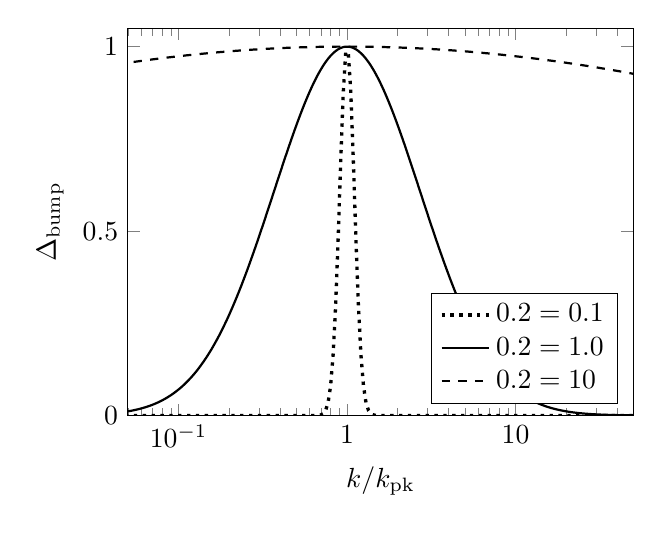
\begin{tikzpicture}
  \def\Abump{1}      % amplitude
  \def\kpk{1}        % k_peak (set to 1 so x is k/k_pk)
  \begin{axis}[
    width=8cm, height=6.5cm,
    xmode=log,
    xmin=5e-2, xmax=5e1,
    ymin=0, ymax=1.05,
    xlabel={$k/k_{\mathrm{pk}}$},
    ylabel={$\Delta_{\mathrm{bump}}$},
    grid=none,
    legend pos=south east,
    legend cell align=left,
    samples=400,
    domain=1e-3:1e3,
    % improve tick formatting on log axis
    xtick={1e-3,1e-2,1e-1,1,1e1,1e2,1e3},
    xticklabels={${10^{-3}}$,$10^{-2}$,$10^{-1}$,$1$,$10$,$10^{2}$,$10^{3}$},
  ]

  % sigma = 0.1
  \addplot[very thick, dotted] { \Abump * exp( - ( (ln(x/\kpk))^2 ) / (2*(0.1)^2) ) };
  \addlegendentry{$\sigma=0.1$}

  % sigma = 1.0
  \addplot[thick] { \Abump * exp( - ( (ln(x/\kpk))^2 ) / (2*(1.0)^2) ) };
  \addlegendentry{$\sigma=1.0$}

  % sigma = 0.5
  \addplot[thick, dashed] { \Abump * exp( - ( (ln(x/\kpk))^2 ) / (2*(10)^2) ) };
  \addlegendentry{$\sigma=10$}

  \end{axis}
\end{tikzpicture}
    \caption{Sigma dependence}
    \label{fig:lognormal_sigma}
\end{subfigure}
\begin{subfigure}[b]{0.45\textwidth}    
    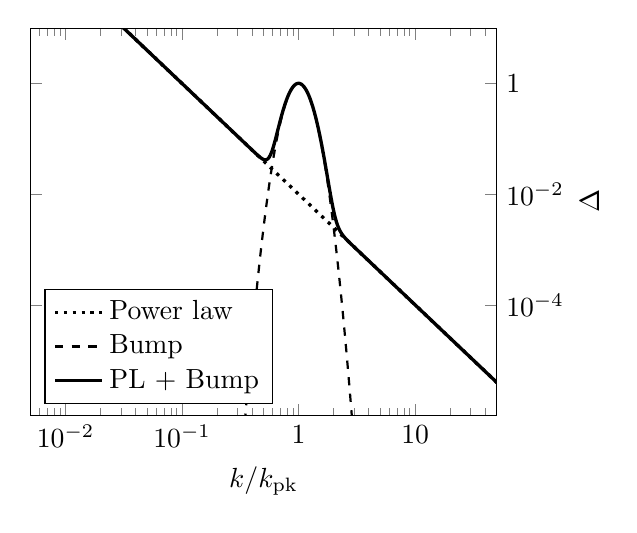
\begin{tikzpicture}
  % --- parameters (edit these) ---
  \def\Abump{1}      % bump amplitude
  \def\kpk{1}        % peak location (so x = k/k_pk)
  \def\sigma{0.2}    % bump width (in ln-space)
  \def\Apl{1e-2}     % power-law amplitude (at k=k_pk)
  \def\npl{-2}       % power-law index: Delta_pl = Apl * (k/k_pk)^npl
  % -------------------------------

  \begin{loglogaxis}[
    width=7.5cm, height=6.5cm,
    xmin=5e-3, xmax=5e1,
    ymin=1e-6, ymax=10,
    xlabel={$k/k_{\mathrm{pk}}$},
    ylabel={$\Delta$},
    grid=none,
    legend pos=south west,
    legend cell align=left,
    samples=800,
    % <- move tick labels to the right
    yticklabel pos=right,
    % <- place ylabel near the right ticks (slightly outside)
    ylabel style={at={(axis description cs:1.2,0.5)},anchor=west},
    xtick={1e-3,1e-2,1e-1,1,1e1,1e2,1e3},
    xticklabels={${10^{-3}}$,$10^{-2}$,$10^{-1}$,$1$,$10$,$10^{2}$,$10^{3}$},
    ytick={1e-4,1e-2,1},
    yticklabels={$10^{-4}$,$10^{-2}$,$1$},
  ]

    % power law
    \addplot[very thick, dotted,domain=1e-3:1e3] { \Apl * (x/\kpk)^(\npl) };
    \addlegendentry{Power law}

    % bump (log-normal in natural log)
    \addplot[thick, dashed, domain=1e-3:1e3] {
      \Abump * exp( - ( (ln(x/\kpk))^2 ) / (2*(\sigma)^2) )
    };
    \addlegendentry{Bump}

    % sum
    \addplot[very thick, domain=1e-3:1e3] {
      \Apl * (x/\kpk)^(\npl) + \Abump * exp( - ( (ln(x/\kpk))^2 ) / (2*(\sigma)^2) )
    };
    \addlegendentry{PL + Bump}

  \end{loglogaxis}
\end{tikzpicture}
\caption{Power spectra comparison}
\label{fig:PS_comp}
\end{subfigure}
\caption{Plots of the power spectra presented in this section. The figure on the left (a) shows the behavior of the bump as $\sigma$ increases: note how a plateau is produced for high values of $\sigma$. The plot on the right (b) compares the power law (dotted) with the bump (dashed) with their sum (solid line). }
\end{figure}

 

